%! TEX root ./master.tex

\lecture{23}{Week 12}{Continue: Coherency Protocols}

\subsection{MOESI}
Compared to the MESI, MOESI added an \textit{Owner} state. 

\begin{itemize}
    \item \textit{Modified}: (same meaning)
    \item \textit{Owner}: there may be several copies of this cache block. We are the only ones who are allowed to modify it but we need to let the others know about the new value.
    \item \textit{Exclusive}: (same meaning)
    \item \textit{Shared}: there may be several copies of this cache block. Only one other process has the right to modify it.
    \item \textit{Invalid}: (same meaning)
\end{itemize}

The owner state allows to share dirty data, additionally to clean cache lines as it it in MESI. So it allows for quickly satisfy read requests for dirty cache blocks without writeback to memory. Accesses to clean data is still done via memory.

This protocol is good if going to remote cache is cheaper than going into main memory.

\paragraph{Invariants}
The MOESI invariants are:

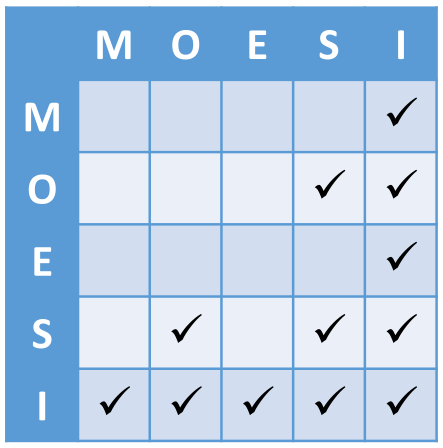
\includegraphics[width=0.8\textwidth]{23_MoesiInvariant.png}

\subsubsection{MESIF}
Compared to MESI, MESIF adds an \textit{Forward} state.

\begin{itemize}
    \item \textit{Modified}: (same meaning)
    \item \textit{Exclusive}: (same meaning)
    \item \textit{Shared}: there may be several copies of this cache block. There is at most one forwarder, whose job is to provided the new line in case it is changed to all others.
    \item \textit{Invalid}: (same meaning)
    \item \textit{Forward}: as shared, but this one is the designated responder for requests.
\end{itemize}

This new forward state allows for cache-to-cache forwards. The new cache block is transferred without memory access.

If there is no forwarder, data is still serverd by main memory. This is even the case if the cache line is shared.

\paragraph{Invariants}
The MESIF invariants are:

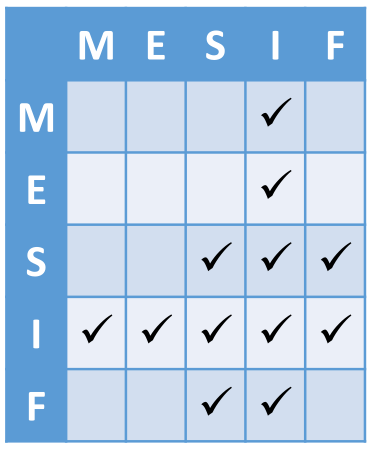
\includegraphics[width=0.8\textwidth]{23_MesifInvariant.png}

\subsubsection{Relaxing Sequential Consistency}
SC required to obtain the program order of processors. But for good performance it is required that we are able to reorder instruction. I.g. Out-of-order execution might reorder instruction, write buffers reorder write instruction, given $a1 < a2$, a1 may be a cache miss while a2 is a cache hit. Also, compilers may reorder or remove reads and writes for performance optimisation reason.

\paragraph{Relaxing Sequential Consistency}
When we relay the requirements for SC, we can make use of the described efficiency gains. There are many different ways to achieve this:
\begin{description}
    \item[Write-to-Read:] later reads can bypass earlier writes
    \item[Write-to-Write:] later writes can bypass earlier writes
    \item[Break write atomicity:] no single visibility order (different processors can see instructions in different orderings)
    \item[Weak ordering:] no implizite order guarantees at all
\end{description}

The more we relaxe the constrains, the less and less guarantees about the model we have and the more and more difficult it gets to reason about modes. But the cheaper and faster implementations we get.

To notify when we need again synchronisation, CPUs provide explicit synchronisation instructions (load fence, memory barrier). I.e. by default CPUs can reorder, but at a certain point (e.g. when entering a critical section) we an request synchronisation.

\paragraph{Processor Consistency}
This is a certain relaxation of SC and it is the default for x86-64. It is also referred to as \textit{Total Store Ordering (TOS)}.

It provides the write-to-read relaxation.This means that all processors see writes from one processor in the order they were issued by that processors. But processors can see many different interleaving of writes from different processors.

This provides a noticeable performance improvement.

\subparagraph{Example}
Recall our earlier example:

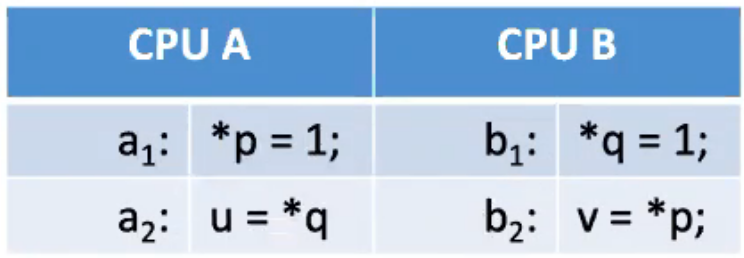
\includegraphics[width=0.8\textwidth]{23_PcEx.png}

Using SC it is not possible to get \code{u = 0, v = 0} but using PC we can get this results. The read instruction a2 can bypass the a1 write resulting in reading $0$ before writing $1$.

\paragraph{Other Consistency Models}
There are also many other relaxations and different architectures support different ones:

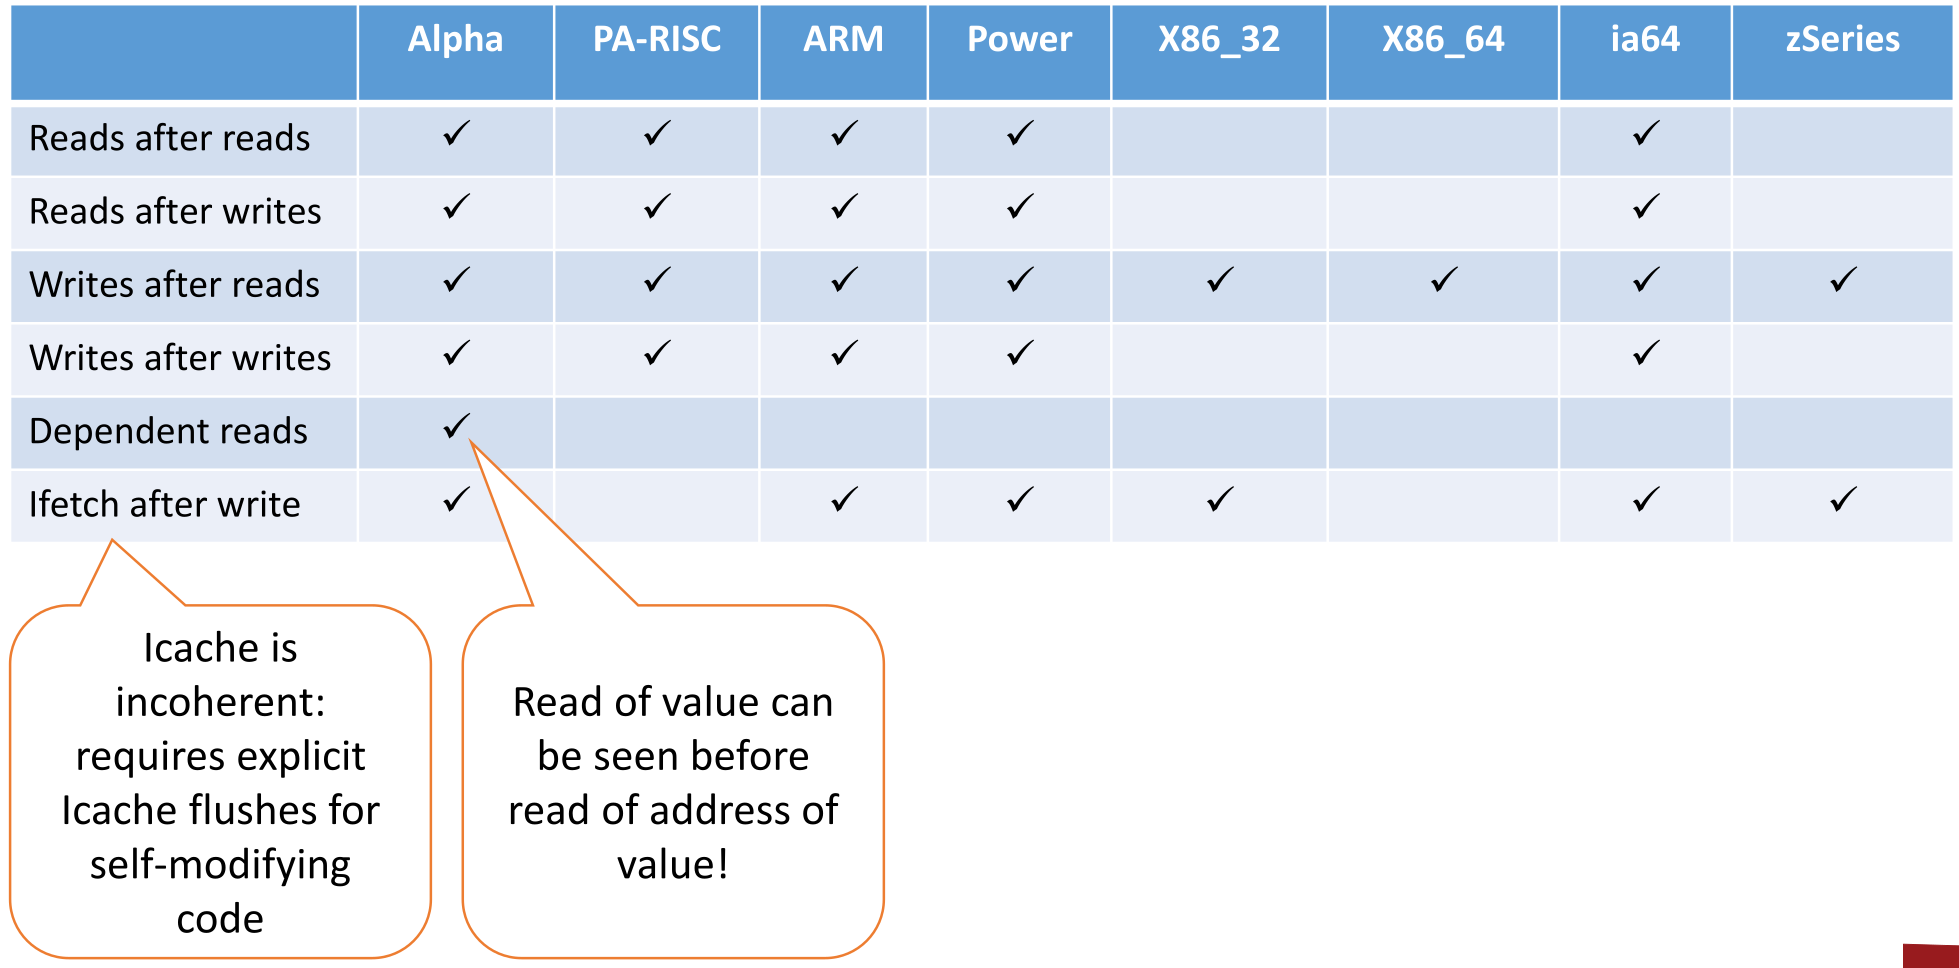
\includegraphics[width=0.8\textwidth]{23_ConsistencyModel.png}

\subsubsection{Barriers and Fences}
\textit{Barriers/fences} provide a way for synchronisation in a weak consistency model. There are two main types:

\paragraph{Compiler Barriers}
Compiler barriers prevent the compiler from reordering memory loads and stores, but they may still reorder register accesses (since they are private to the compiler). In gcc we would use \code{__asm__ __volatile__("" ::: "memory");} to tell the gcc compiler to use such a barrier. This code is called compiler intrinsic.

\paragraph{Memory Barriers}
Memory barriers prevent the CPU from reordering load/store instructions before a barrier with load/store instructions after a barrier. They are like a \textit{wall} for instructions. For this the \code{MFENCE} instruction is used.

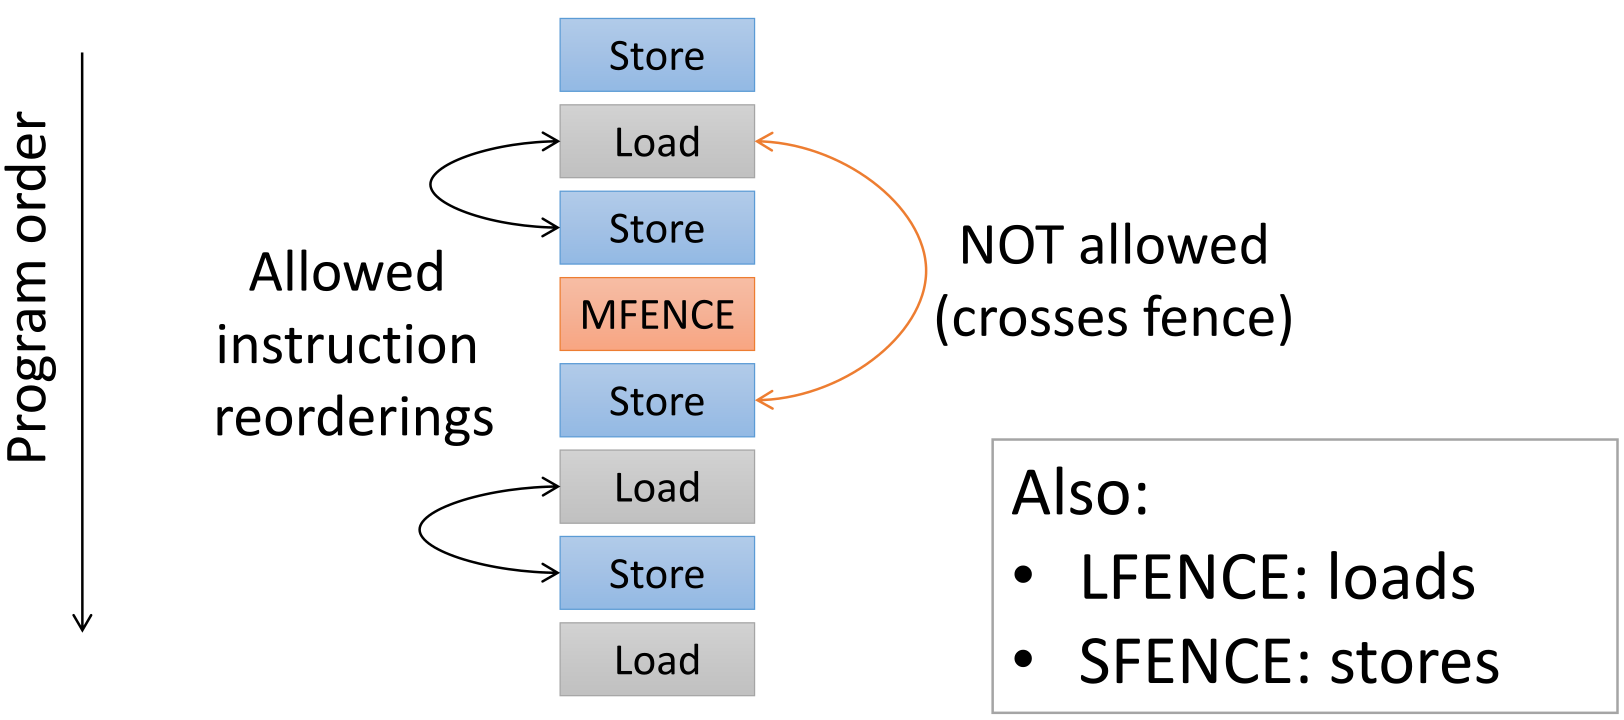
\includegraphics[width=0.8\textwidth]{23_MemoryBarriers.png}

There are also fences for only stores \code{LFENCE} and store \code{SFENCE}.

\subsubsection{Multicore Synchronisation: Test-and-Set}
There are two different ways so synchronize across processors:

\begin{itemize}
    \item \textit{Atomic operations}: Allow doing a series of operations without interruption by other processes
        \begin{itemize}
            \item e.g. test-and-set, compare-and-swap
        \end{itemize}
    \item \textit{Interprocessor Interrups}: when processors interrupt each other. This is e.g. used in OSs (not really part of this course)
\end{itemize}

\paragraph{Test-And-Set (TAS)}
TAS is one of the simplest non-trivial atomic registers and is is implemented in HW. Firstly, we read value stored at a certain memory location into a register. Then we store $1$ into that location. This is all done atomically. So the memory bus must be blocked in the meantime.

\subsubsection{Spinlock}
We can use TAS to implement a spinlock. To acquire a mutex we use

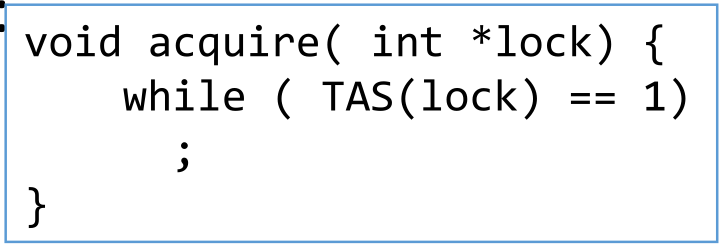
\includegraphics[width=0.8\textwidth]{23_TasSpinlockAqu.png}

and to release it, we simple set it back to $0$

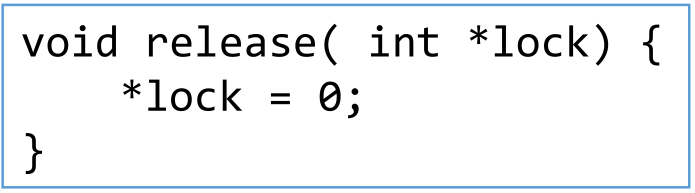
\includegraphics[width=0.8\textwidth]{23_TasSpinlockRel.png}

\code{TAS(someAddr)} reads the value which is at \code{someAddr} and then writes $1$ into the lock. After, the read value is returned.

In the case when $1$ is returned, we know that the lock is already locked and hence we retry till we get a $0$.

This is only efficient if we know that there are not many processes waiting for the mutex and that a lock is only keeps for a short amount of time, because

\begin{itemize}
    \item memory must be locked while lock is locked
    \item atomically read and write memory over and over
    \item busy waiting requires CPU usage
\end{itemize}

\paragraph{Test And Test-And-Set}
This provides great improvements over the normal TAS. The inner while loop is not done atomically and it does also not involve any writes. Therefore, it is rather cheap to busy loop here. The expensive TAS is only done when the inner while loop detects that there is a chance of being successful.

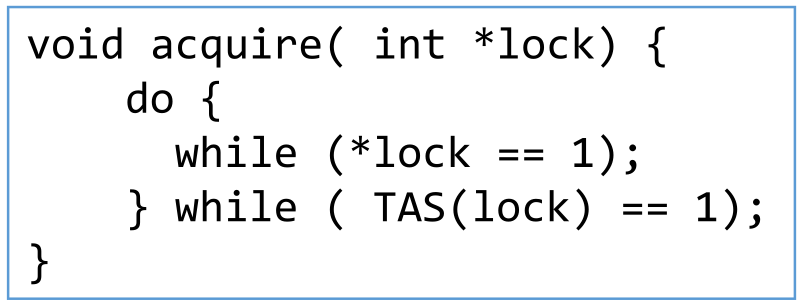
\includegraphics[width=0.8\textwidth]{23_TestAndTestAndSet.png}

In general, we should not use this in practice. Compilers and processors may reorder the instructions and the memory consistency may break the code's semantics too. While TAS is implemented in HW, Test and TAS is not.

\subsubsection{Compare and Swap}
This is another atomic operations. It is more complex than TAW but also more powerful. It is commonly used for wait-free data structures. It takes three parameters, a address and two values:

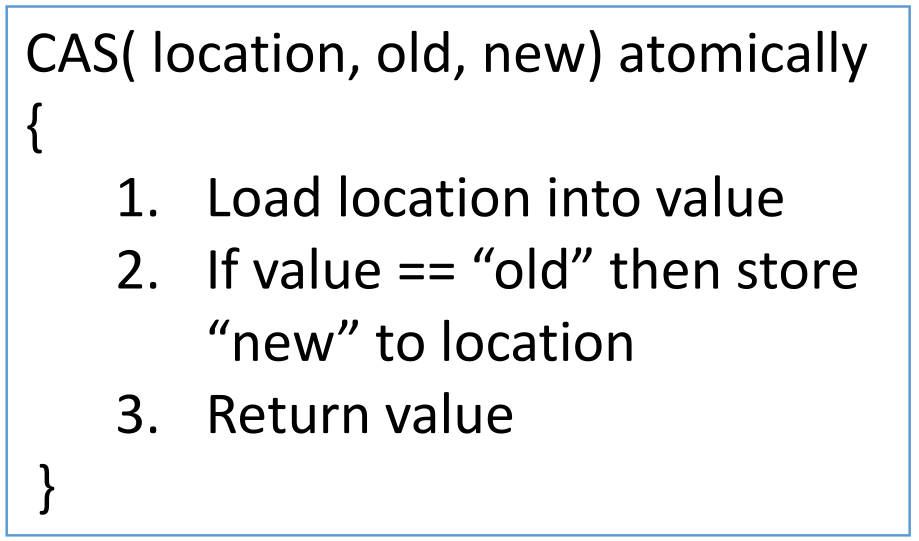
\includegraphics[width=0.8\textwidth]{23_CompareAndSwap.png}

Often, the location is a pointer and we need to update where the pointer points to.

\paragraph{CAS Lock-Free Update}
In general we do a copy of the DS which we modify. When none has changed the original one, we make our copy the new original. The CAS is used on the pointer.

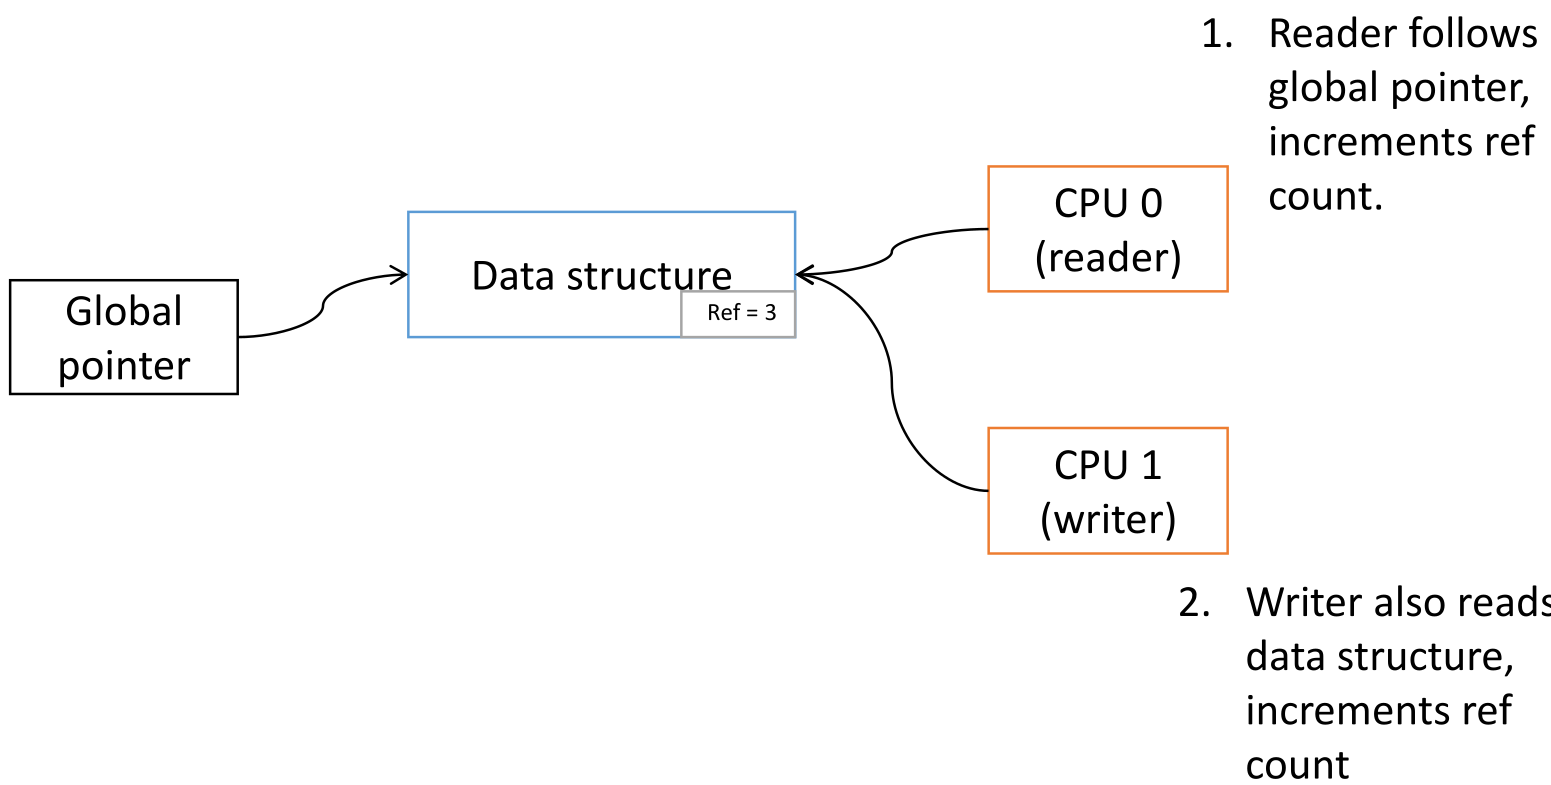
\includegraphics[width=0.8\textwidth]{23_CasEx1.png}

Given a DS, a reader and a write. \code{Ref} is the reference count to the DS. The reader increments the ref and starts reading. The writer increments the ref, copies the DS, decrement the ref and then modifies it. When done, it wants to make the copied DS the new original one.

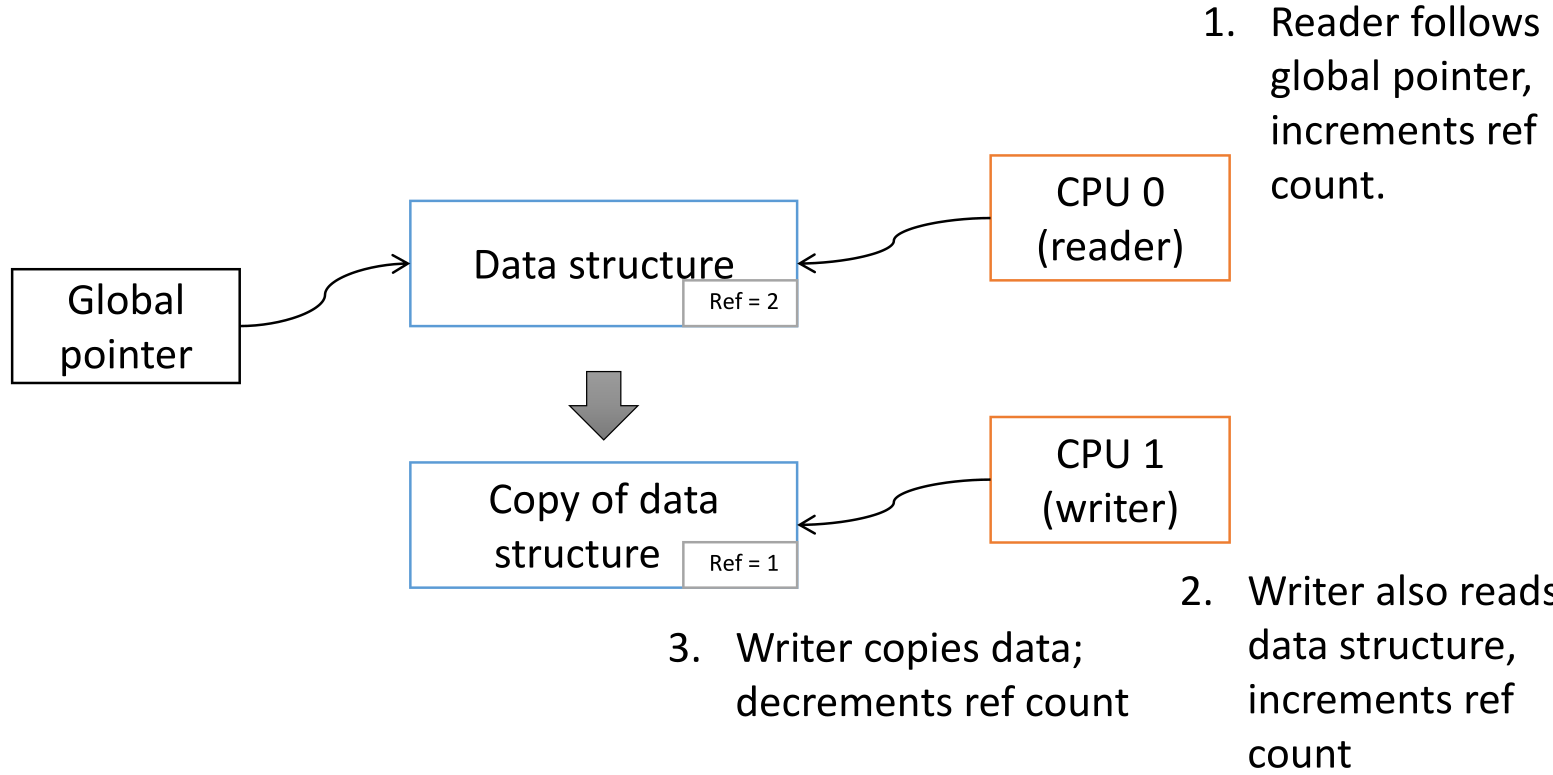
\includegraphics[width=0.8\textwidth]{23_CasEx2.png}

Using CAS, we adjust the global pointer to point to our new copy, as long as the global pointer did not change between making our copy and storing our copy.

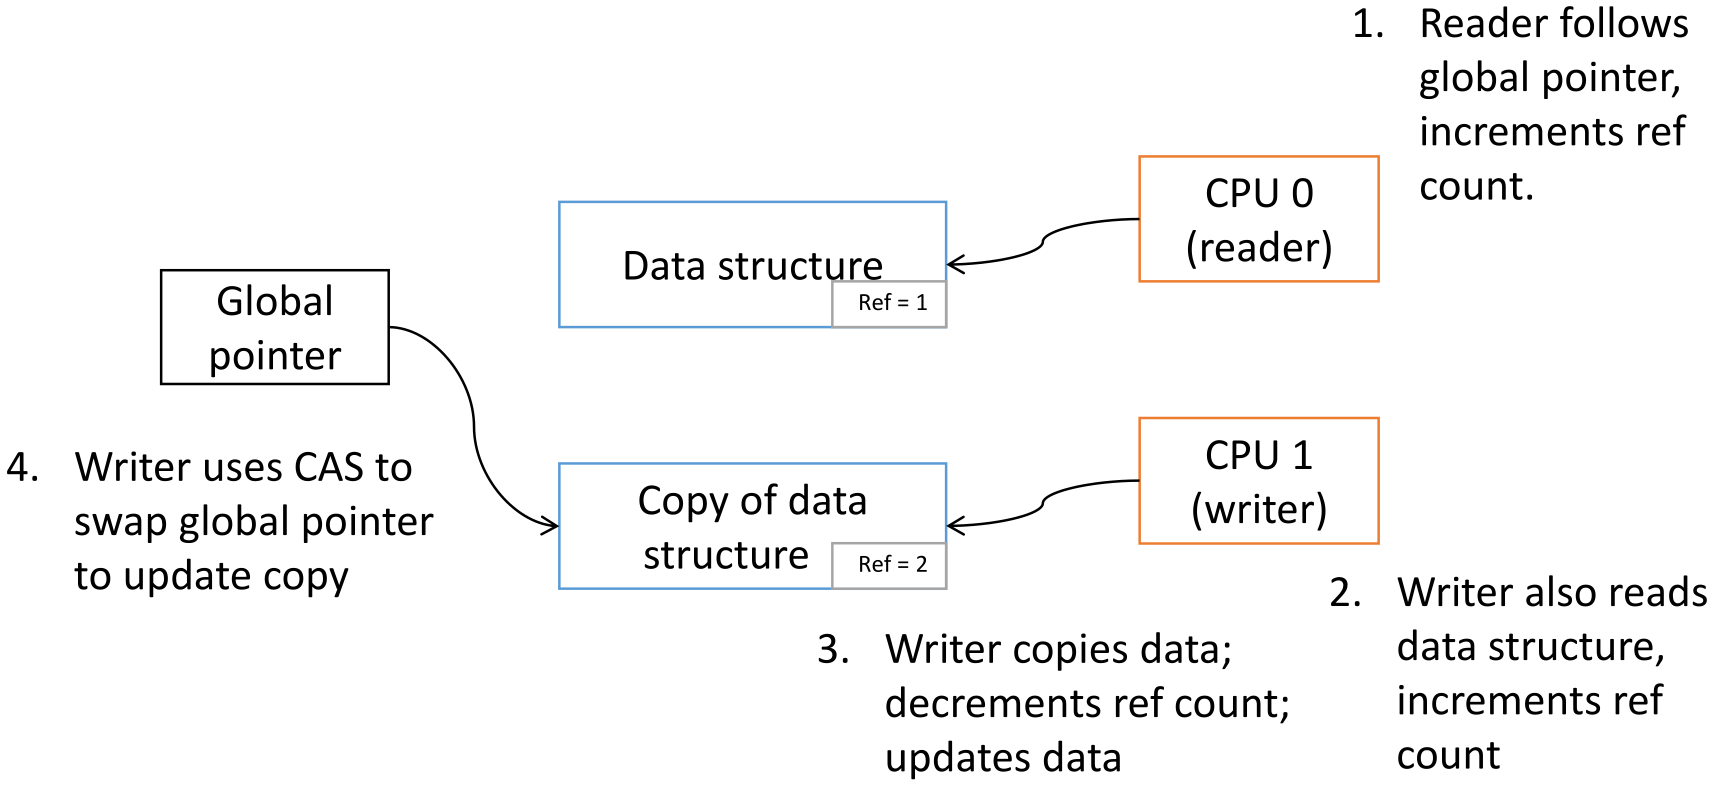
\includegraphics[width=0.8\textwidth]{23_Cas_Ex3.png}

After global pointer is updated and there are no reader to the old original anymore, the old original id discarded.

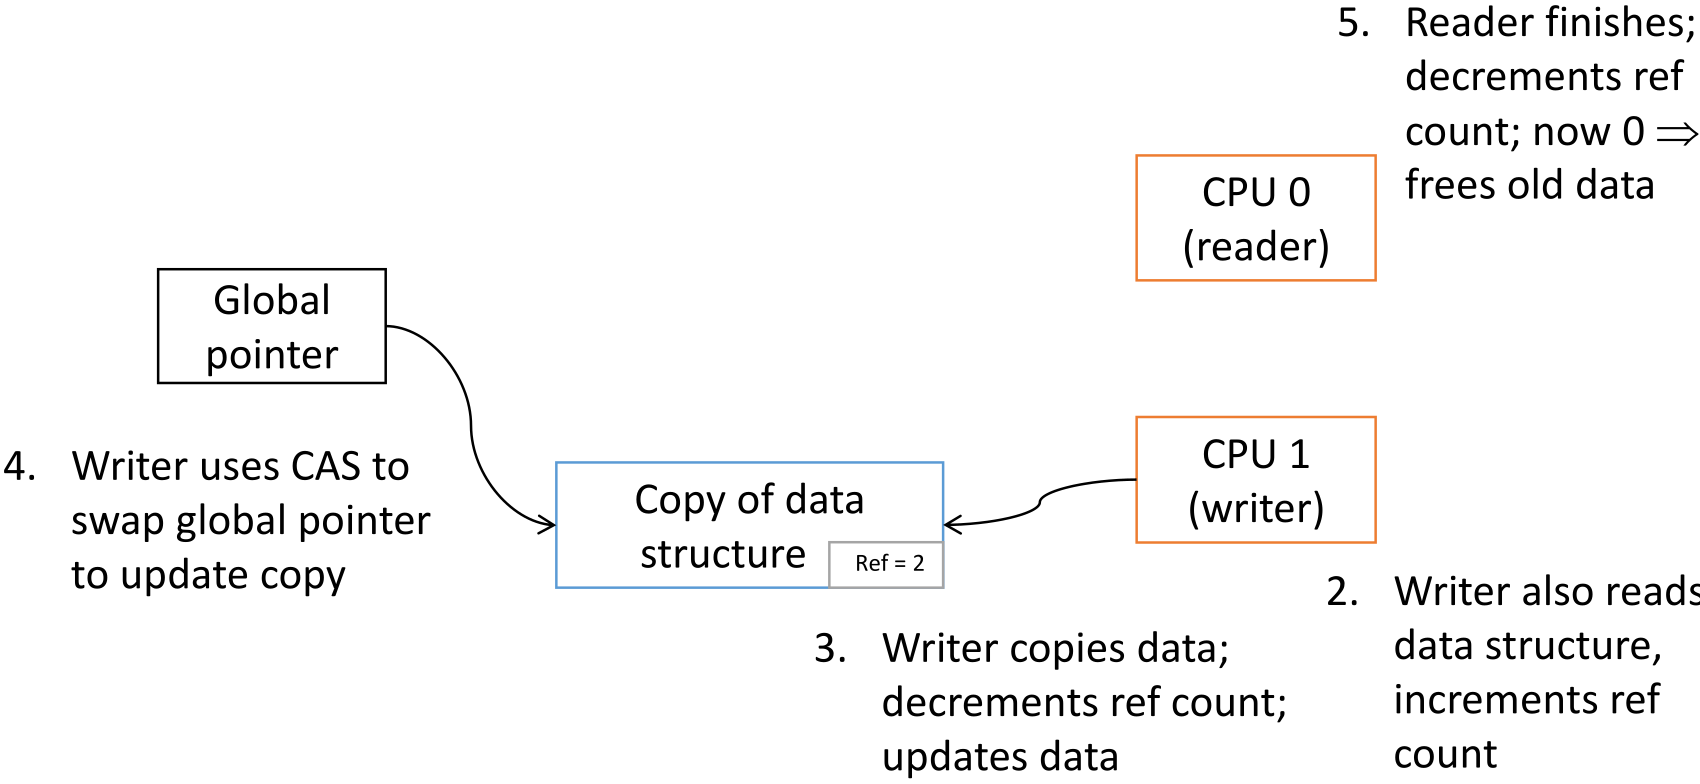
\includegraphics[width=0.8\textwidth]{23_CasEx4.png}

When the write finishes, we decrement the ref

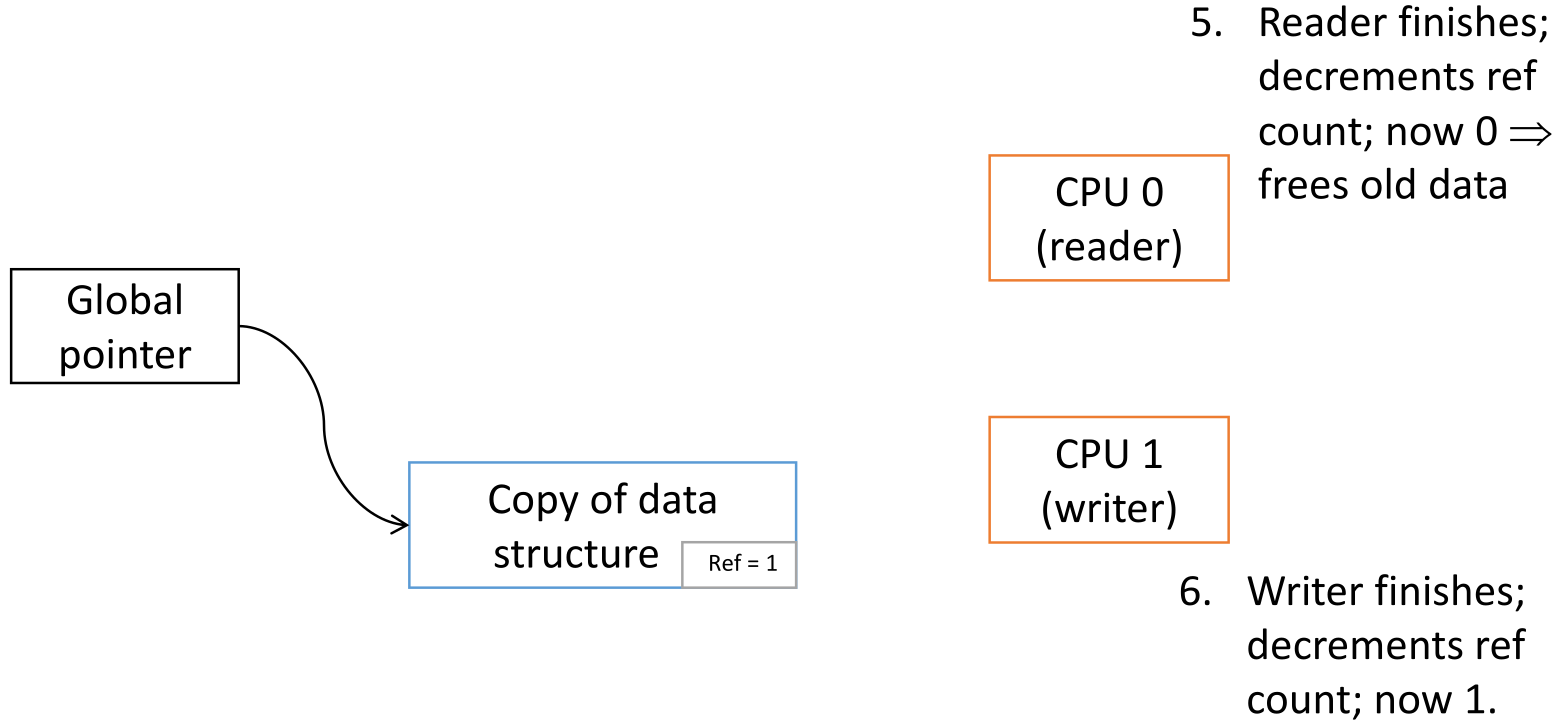
\includegraphics[width=0.8\textwidth]{23_CasEx5.png}

\paragraph{ABA-Problem}
The problem with CAS is, that when there is a change to the value, and the another change, which changes it back to the initial value, we cannot detect that there was actually a change in the meantime:

\begin{itemize}
    \item A reads value as x
    \item B write y to value
    \item B writes x as value
    \item A reads value as x and wrongly assumes it is untouched
\end{itemize}

Sometimes this is not really an issue, but sometimes it can break everything.

I.e. the value did not change while the data changed. To solve this, we must ensure that the value always changes. This can be done e.g. by splitting the value into the original value and an increasing counter. 

\paragraph{Double Compare-And-Swap}
Double CAS, aka CAS2 or DCAS takes not only $3$ arguments, but $6$. It takes two memory locations, two times the old data and two times the new data. Then it does (atomically):
\begin{enumerate}
    \item Compare the memory locations
    \item If both match, each is updated with a different new value
    \item If not, the existing values in the locations are loaded
\end{enumerate}

This is is claimed to be more powerful than CAS, it is rarely implemented tue to its complexity.

\subsubsection{x86}
On this architecture we have:

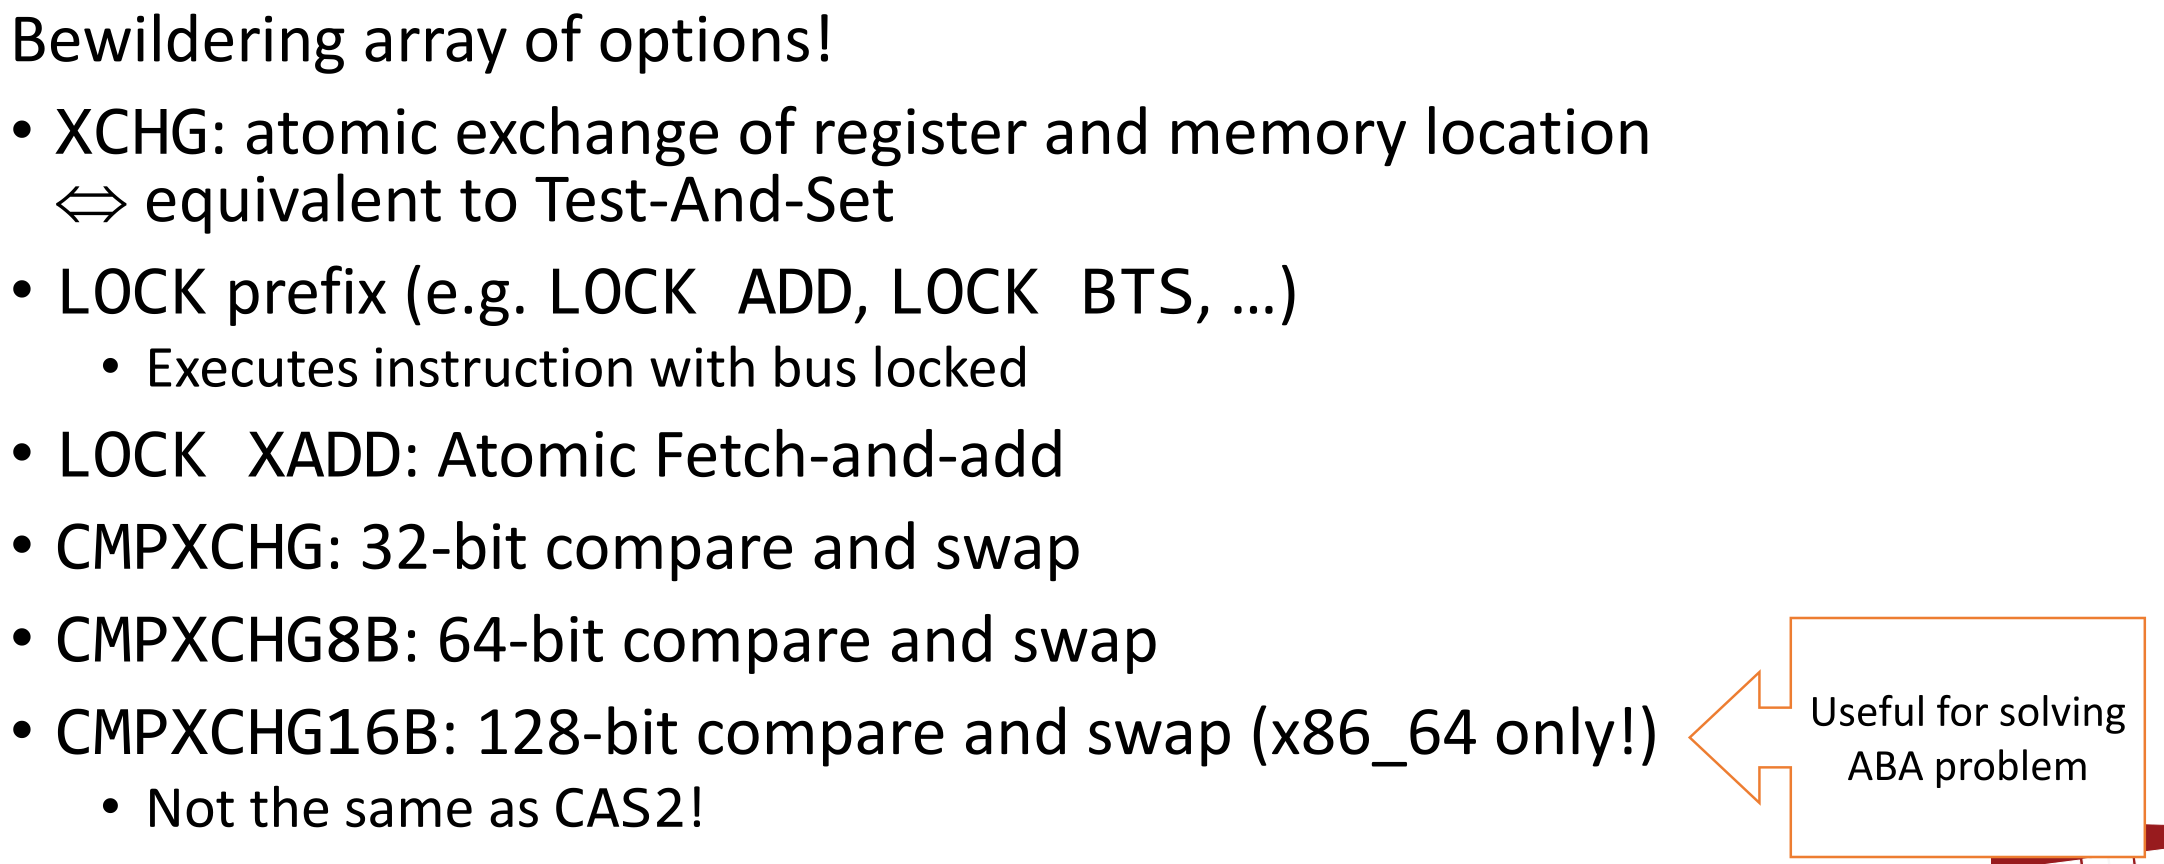
\includegraphics[width=0.8\textwidth]{23_x86Summary.png}

Atomiv exchange of registers is pretty much TAS.

\subsubsection{Simultaneous Multithreading}
This is called hyperthreading too (by intel).

\paragraph{SMP Performance Limits}
Memory is the bottleneck for cache-coherent SMPs. All accesses to main memory stall the processor. While MOESI allows to cache-to-cahce transfer, cache themselves can be slow too. Stalls caused by memory asses will most likely halt the complete processor (unless we can extract enough ILP).

\paragraph{Simultaneous Multithreading}
Many parts of the CPU are idle at a given time and many instructions do not required the memory units. But ILP is very limited. It there a way to make use of the processor while it is waiting for memory? The question arises if we cannot use the superscalar idea to make use of idle parts of a stalled core of a multicore CPU.

\paragraph{Types of MT}
There are three types of multithreading.

A color represents works of a certain process, white boxes are ones which could not be filled due to low ILP

\begin{description}
    \item[Coarse-gain MT:] We switch the thread as soon as we hit a time consuming instruction, e.g. a cache miss.
    \item[Fine-Grain MT:] We switch the thread much more often, e.g. after each instruction.
    \item[SMT:] In the same cycle we execute instructions of different threads.
\end{description}

\paragraph{In Practice}
A modern CPU has often two hyperthreads per code and they are exposed to the OS as separate threads. Therefore, the OS tells us that we have twice the number of threads than we actually have.

\paragraph{Advantages/Disadvantages}
It is not always a win, but it provided 10 to 20 percent performance boost and it is rather cheap since the hardware is already there. Tough in practice, two physical cores are more performant than two hyperthreads (running on the same core) (which is not very surprising). Hyperthreading can be disabled.
